\documentclass[../main.tex]{subfiles}

\begin{document}

\chapter{安装}
\vspace{-2cm}

本章节首先介绍安装 BasicSR 所需的环境依赖 (第\ref{installation:env-reqirement}小节),随后介绍安装 BasicSR 的两种方式:本地 clone 源代码安装和 pip 安装 basicsr 包 (第\ref{installation:install}小节)。对于需要在项目中使用 PyTorch C++ 编译算子的情况,我们也提供了相应的安装方式 (第\ref{installation:c++}小节)。
最后,我们将安装过程中的常见问题进行了汇总 (第\ref{installation:faq}小节)。

\section{环境依赖}
\label{installation:env-reqirement}

由于 BasicSR 是基于 \href{https://www.python.org/}{Python} 语言和 \href{https://pytorch.org/}{PyTorch} 深度学习框架进行开发的,因此在安装 BasicsR 之前,需要在电脑或者服务器上安装 Python 环境以及各种相关的 Python 库;如果想要在 \textbf{GPU} 上运行程序的话,也需要先在电脑上配置相应的 CUDA 环境。以下我们分别对 CUDA 和相应的 Python 库进行简要说明。

\begin{enumerate}
    \item NVIDIA GPU + \href{https://developer.nvidia.com/cuda-downloads}{CUDA}:GPU (Graphics Processing Unit) 由于其高效的并行能力,目前被广泛用于深度学习的计算中;CUDA (Compute Unified Device Architecture) 是 NVIDIA 推出的可以让 GPU 解决复杂计算问题的运算平台。如果需要训练 BasicSR 中的模型,需要使用 GPU 并配置好相应的 CUDA 环境。
    \item Python 和 Python 库 (对于 Python 库,我们提供了相应的安装脚本):
    \begin{enumerate}
        \item Python >= 3.7 (推荐使用\href{https://www.anaconda.com/products/distribution#linux}{Anaconda}或者\href{https://docs.conda.io/en/latest/miniconda.html}{Miniconda})
        \item \href{https://pytorch.org/}{PyTorch >= 1.7}:目前深度学习领域广泛使用的深度学习框架
    \end{enumerate}
\end{enumerate}

当配置好 Python 环境和 CUDA 环境之后,可以直接运行以下的脚本一次性安装 BasicSR 中调用的各种 Python 库:

\begin{minted}[xleftmargin=20pt,bgcolor=bg]{bash}
pip install -r requirements.txt
\end{minted}

\begin{note} % ---------------- Note block ---------------- %
    \textbf{Windows 环境}

    BasicSR 也支持 Windows 环境。

    更多注意事项,参见第\ref{installation:faq}小节 Q1 问题。
\end{note}

\section{BasicSR 安装}
\label{installation:install}
在安装好上述的环境依赖后,此时就可以进行 BasicSR 的安装了。

本小节的安装默认不适用 PyTorch C++ 编译算子,若需要,则参考第 \ref{installation:c++} 小节进行安装。

\begin{hl} % ---------------- Highlight block ---------------- %
    \textbf{BasicSR 安装方式}

    根据不同的需求,我们提供了两种安装 BasicSR 方式,{\color{red}\textbf{两种方式只能选择一种安装,否则容易产生冲突}}。

    \begin{itemize}
        \item 如果希望\textbf{查看 BasicSR 中的细节}或者需要对其进行\textbf{修改},推荐通过本地 clone 代码的方式进行安装。
        \item 如果仅仅是将 BasicSR 作为一个\textbf{ Python 包}进行使用 (比如 项目 \href{https://github.com/TencentARC/GFPGAN}{GFPGAN} 和 \href{https://github.com/xinntao/Real-ESRGAN}{Real-ESRGAN}),推荐直接从 PyPI 安装 BasicSR,这样可以使得自身项目的代码结构更加简洁。
    \end{itemize}
\end{hl}

\subsection{本地 clone 代码}
\label{installation:local-clone}
要通过本地 clone 安装 BasicSR,需要在终端上依次进行以下3个步骤。

\begin{enumerate}
    \item 克隆项目:
    \begin{minted}[xleftmargin=20pt,bgcolor=bg]{bash}
git clone https://github.com/XPixelGroup/BasicSR.git
    \end{minted}

    \item 安装依赖包:
    \begin{minted}[xleftmargin=20pt,bgcolor=bg]{bash}
cd BasicSR
pip install -r requirements.txt
    \end{minted}

    \item 在 BasicSR 的根目录下安装 BasicSR:
    \begin{minted}[xleftmargin=20pt,bgcolor=bg]{bash}
python setup.py develop
    \end{minted}
\end{enumerate}

如果希望安装的时候指定 CUDA 路径,可使用如下指令:

\begin{minted}[xleftmargin=20pt,bgcolor=bg]{bash}
CUDA_HOME=/usr/local/cuda \
CUDNN_INCLUDE_DIR=/usr/local/cuda \
CUDNN_LIB_DIR=/usr/local/cuda \
python setup.py develop

\end{minted}

\subsection{pip 安装}
\label{installation:pip-install}
对于使用 pip 安装 BasicSR,在终端上运行以下指令即可:
    \begin{minted}[xleftmargin=20pt,bgcolor=bg]{bash}
pip install basicsr
    \end{minted}

如果希望安装的时候指定 CUDA 路径,可使用如下指令:

\begin{minted}[xleftmargin=20pt,bgcolor=bg]{bash}
CUDA_HOME=/usr/local/cuda \
CUDNN_INCLUDE_DIR=/usr/local/cuda \
CUDNN_LIB_DIR=/usr/local/cuda \
pip install basicsr
\end{minted}

\subsection{验证 BasicSR 是否安装成功}

当选择了上述两种方式中的一种方式安装 BasicSR 后,我们可以通过图\ref{fig:correct-install}的方式来判断是否成功安装 BasicSR:

\begin{figure}[H]
%\vspace{-0.5cm}
\begin{center}
    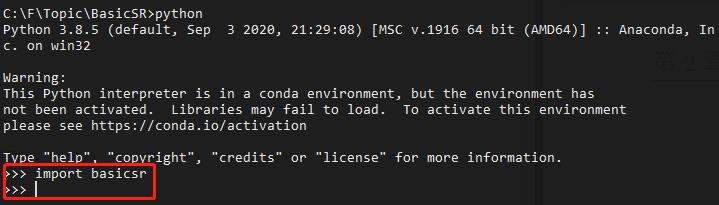
\includegraphics[width=0.9\linewidth]{figures/installation_correct_install.jpg}
    \caption{验证成功安装 BasicSR}
    \label{fig:correct-install}
\end{center}
\vspace{-0.5cm}
\end{figure}

如果此时没有报错,则说明 BasicSR 安装成功,此时便可以基于 BasicSR 进行开发啦 $\sim \sim \sim$

\section{PyTorch C++ 编译算子}
\label{installation:c++}

考虑到某些项目中会需要使用 PyTorch C++ 编译算子,我们在这个小节针对这种情况也提供了相应的 BasicSR 安装方式。如果不需要使用相关 C++ 编译算子,则此小节可以跳过。

对于项目中需要使用以下的 PyTorch C++ 编译算子时,比如:

\begin{itemize}
    \item 可变性卷积 DCN (如果安装的 Torchvision 版本 >= 0.9.0,会自动使用 TorchVision 中提供的 DCN,故不需要安装此编译算子),比如:\href{https://github.com/XPixelGroup/BasicSR/tree/master/basicsr/ops}{EDVR 中的 DCN}

    \item StyleGAN 中的特定的算子,比如:\href{https://github.com/XPixelGroup/BasicSR/tree/master/basicsr/ops}{upfirdn2d, fused\_act}
\end{itemize}

由于第\ref{installation:install}小节所提到的安装方式不支持 PyTorch C++ 编译算子,为了能够使用 PyTorch C++ 编译算子,此时需要一些特定的修改 (有以下两种方式可供选择):

\begin{enumerate}
    \item \textbf{安装}的时候对 PyTorch C++ 编译算子进行编译:此时需要将原先的安装指令进行修改,其中 \texttt{BASICSR\_EXT=True} 中的 \texttt{EXT} 是单词 Extension 的缩写。
    \begin{enumerate}
        \item 对于通过本地 clone 代码安装 BasicSR 的方式,此时修改指令:
        \begin{minted}[xleftmargin=20pt,bgcolor=bg]{bash}
python setup.py develop --> BASICSR_EXT=True python setup.py develop
        \end{minted}
        \item 对于通过 pip 安装 BasicSR 的方式,此时修改指令:
        \begin{minted}[xleftmargin=20pt,bgcolor=bg]{bash}
pip install basicsr --> BASICSR_EXT=True pip install basicsr
        \end{minted}
    \end{enumerate}
    进行了上述的修改之后,如果我们需要运行 StyleGAN 的测试代码 (需要用到 PyTorch C++ 编译算子) (代码位于 \href{https://github.com/XPixelGroup/BasicSR/blob/master/inference/inference_stylegan2.py}{inference/inference\_stylegan2.py}),此时直接输入指令即可:
    \begin{minted}[xleftmargin=20pt,bgcolor=bg]{bash}
python inference/inference_stylegan2.py
        \end{minted}

    \item \textbf{每次在跑程序}的时候\textbf{即时加载 (JIT)} PyTorch C++ 编译算子:如果我们选择了这种方式,此时不需要修改 BasicSR 的安装指令。依然拿 StyleGAN 的测试代码举例,在这种情况下,如果想要运行 StyleGAN 的测试代码,此时需要输入的指令是:
    \begin{minted}[xleftmargin=20pt,bgcolor=bg]{bash}
BASICSR_JIT=True python inference/inference_stylegan2.py
    \end{minted}

\end{enumerate}

关于上述提到的两种使用 PyTorch C++ 编译算子方式之间的优劣和场景对比如表\ref{tab:env}所示:

\begin{table}[h]
\centering
\footnotesize
\begin{tabular}{|c|c|c|c|c|}
  \hline
  选项                     & 优点                  & 缺点                            & 适用场景         & 具体安装指令 \\
  \hline
  \textbf{安装}编译 C++ 算子 & \makecell[c]{运行代码的时候, \\ 能够快速加载编译算子} & \makecell*[c]{配置环境的时候, \\ 需要更多的依赖,\\碰到的问题可能更多} & \makecell[c]{需要多次训练或 \\ 多次测试模型} & \makecell[c]{在安装的时候,设置 \\\textbf{BASICSR\_EXT=True}}\\
  \hline
  \textbf{即时加载} C++ 算子 & \makecell[c]{有着更少的依赖,\\碰到的问题可能更少} & \makecell[c]{每次运行代码的时候,\\都需要花费几分钟\\重新编译算子} & 仅仅是进行测试 & \makecell[c]{在跑程序的时候,设置 \\\textbf{BASICSR\_JIT=True}} \\
  \hline
\end{tabular}
\caption{\label{tab:env}安装编译算子和即时加载编译算子的对比。}
\end{table}

\begin{note} % ---------------- Note block ---------------- %
\textbf{注意}
\begin{enumerate}
     \item 对于需要在安装的时候就编译 PyTorch C++ 算子,需要确保:gcc 和 g++ 版本 >= 5。
     \item \texttt{BasicSR\_JIT} 有最高的优先级。即使在安装的时候已经成功编译了 C++ 编译算子,若在运行代码指令中设置了 \texttt{BasicSR\_JIT=True},此时代码仍旧会即时加载 C++ 编译算子。
     \item 在\textbf{安装}的时候,不能设置 \texttt{BasicSR\_JIT=True}。
\end{enumerate}
\end{note}

\section{常见安装问题}
\label{installation:faq}

\begin{enumerate}
    \item \textbf{Q1: Windows 下是否可以使用?}

    经过验证,Windows 下可以通过上述的两种安装方式安装 BasicSR。如果需要使用 CUDA,需要指定 CUDA 路径。	另外需要注意的是如果需要在 Windows 环境中使用环境变量,需要使用以下方式:
       \begin{minted}[xleftmargin=20pt,bgcolor=bg]{bash}
set BASICSR_EXT=True
       \end{minted}

    由于 BasicSR 项目是在 Linux (Ubuntu) 环境下进行开发的,因此推荐在 Linux 环境下基于 BasicSR 进行项目的开发。

    \item \textbf{Q2: \texttt{BASICSR\_EXT} 和 \texttt{BASICSR\_JIT} 在什么环境下才能执行?}

    如果在加入 \texttt{BASICSR\_EXT} 和 \texttt{BASICSR\_JIT} 环境变量之后运行报错,此时需要检查 gcc 版本。BasicSR 在已被验证在 gcc5 $\sim$ gcc7 版本下可以成功编译 C++ 编译算子。

    \item \textbf{Q3: 安装路径混淆的问题}

    很多问题都是由于安装路径混淆,其主要原因是本地 clone 代码和 pip 安装包两个方式被同时执行。

    具体而言,如果先通过 pip 安装了 BasicSR,随后又使用本地 clone 的方式进行安装,此时项目中调用的 BasicSR 路径还是 pip 安装的 BasicSR;反过来,如果先使用本地 clone 的方式进行安装,随后又使用 pip 安装,此时项目中调用的 BasicSR 路径还是本地 clone 下的BasicSR (分别如图\ref{fig:false-clone-install}和图\ref{fig:false-pip-install}所示)。

\begin{enumerate}
    \item 通过本地 clone 安装成功的时候,此时使用 \texttt{pip list} 命令查看 basicsr 路径:
    \begin{figure}[H]
    %\vspace{-0.5cm}
    \begin{center}
        %\fbox{\rule{0pt}{2.5in} \rule{0.9\linewidth}{0pt}}
        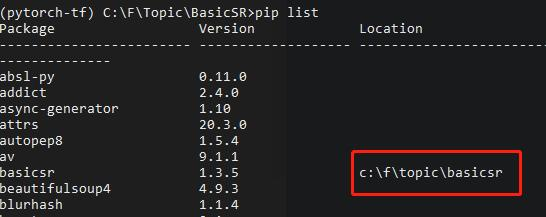
\includegraphics[width=0.7\linewidth]{figures/installation_clone_install_location.jpg}
        \caption{本地 clone 安装成功时的 basicsr 路径显示}
        \label{fig:correct-clone-install}
    \end{center}
    \vspace{-0.5cm}
    \end{figure}

    \item 通过 pip 安装成功的时候,此时使用 \texttt{pip list} 命令查看 basicsr 路径:
    \begin{figure}[H]
    %\vspace{-0.5cm}
    \begin{center}
        %\fbox{\rule{0pt}{2.5in} \rule{0.9\linewidth}{0pt}}
        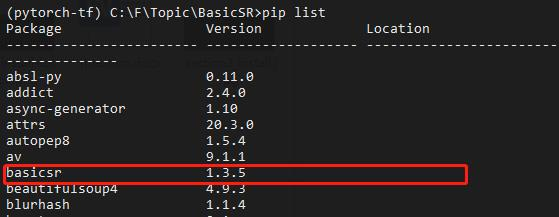
\includegraphics[width=0.7\linewidth]{figures/installation_pip_install_location.jpg}
        \caption{pip 安装成功时的 basicsr 路径显示 (如果指向 anaconda 下的路径,也是正常的)}
        \label{fig:correct-pip-install}
    \end{center}
    \vspace{-0.5cm}
    \end{figure}

    \item 如果先通过 pip 安装,随后通过本地 clone 安装,此时使用 \texttt{pip list} 命令查看 basicsr 路径:
    \begin{figure}[H]
    %\vspace{-0.5cm}
    \begin{center}
        %\fbox{\rule{0pt}{2.5in} \rule{0.9\linewidth}{0pt}}
        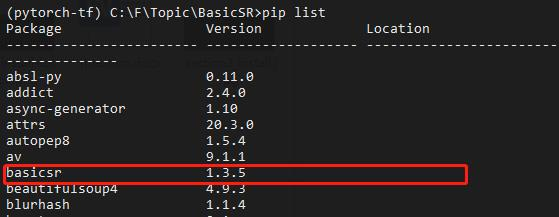
\includegraphics[width=0.7\linewidth]{figures/installation_pip_install_location.jpg}
        \caption{basicsr 路径并未指向本地 clone 的 BasicSR}
        \label{fig:false-clone-install}
    \end{center}
    \vspace{-0.5cm}
    \end{figure}

    \item 如果先通过本地 clone 安装,随后通过 pip 安装,通过 \texttt{pip list} 命令查看此时 basicsr 路径:
    \begin{figure}[H]
    %\vspace{-0.5cm}
    \begin{center}
        %\fbox{\rule{0pt}{2.5in} \rule{0.9\linewidth}{0pt}}
        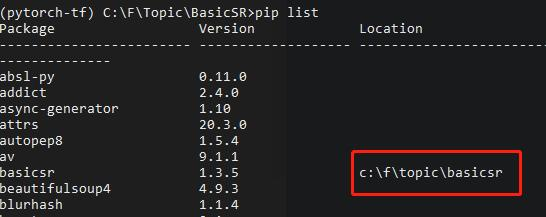
\includegraphics[width=0.7\linewidth]{figures/installation_clone_install_location.jpg}
        \caption{basicsr 路径并未指向 python 环境下 (或者 anaconda) 下 的 BasicSR}
        \label{fig:false-pip-install}
    \end{center}
    \vspace{-0.5cm}
    \end{figure}

\end{enumerate}
    对于上述的两种错误情况 (图\ref{fig:false-clone-install}和图\ref{fig:false-pip-install}),此时正常的解决方式为:先将安装的 BasicSR 进行卸载,随后再根据项目的需要重新选择一种方式安装 BasicSR。
\begin{minted}[xleftmargin=20pt,bgcolor=bg]{bash}
pip uninstall basicsr
\end{minted}

    \item \textbf{Q4: 如何更新最新版本的 BasicSR?}

\begin{enumerate}
    \item 对于通过本地 clone 进行安装的方式,需要将本地的 BasicSR 项目代码与\href{https://github.com/XPixelGroup/BasicSR}{远端的 BasicSR 项目代码}进行同步。
    \item 对于通过 pip 安装的方式,
    \begin{minted}[xleftmargin=20pt,bgcolor=bg]{bash}
pip install basicsr --upgrade
    \end{minted}
\end{enumerate}

    \item \textbf{Q5: 如何解决运行代码时出现的 version 问题?}

    有时候在运行代码的时候,会出现类似于如下的问题:
    \begin{figure}[H]
    %\vspace{-0.5cm}
    \begin{center}
        %\fbox{\rule{0pt}{2.5in} \rule{0.9\linewidth}{0pt}}
        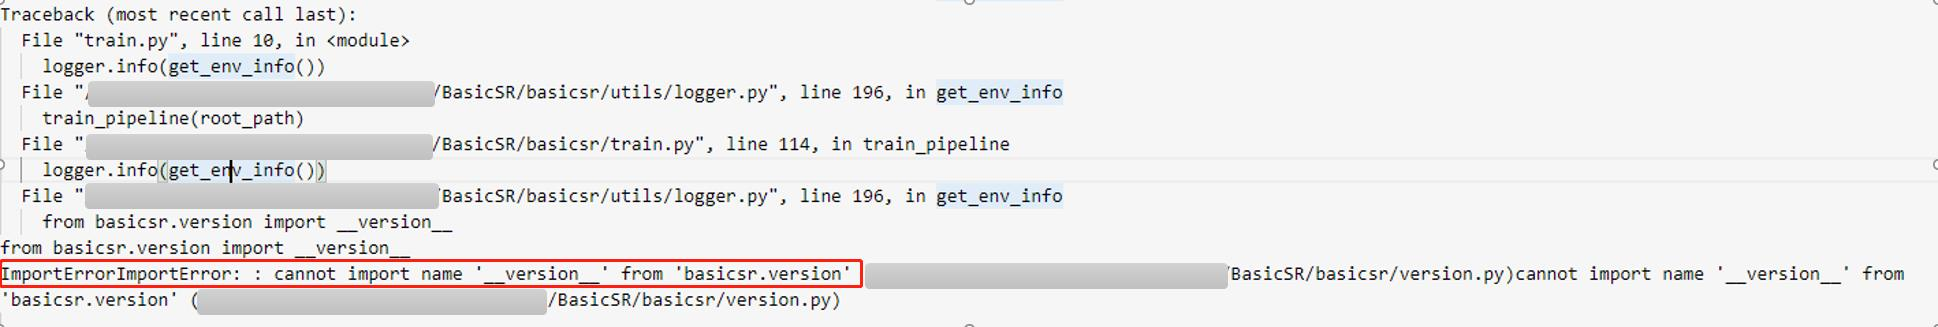
\includegraphics[width=0.8\linewidth]{figures/installation_version.jpg}
        \caption{version问题示例}
        \label{fig:version}
    \end{center}
    \vspace{-0.5cm}
    \end{figure}
    此时,可以尝试:
    \begin{enumerate}
        \item 重新运行安装 BasicSR 的指令。
        \item 将涉及到 version 的代码进行注释。
    \end{enumerate}

\end{enumerate}

\begin{hl}
    如果小伙伴们在安装过程中还遇到其它的问题,可以在我们的 BasicSR 微信群、 QQ 群 (可从 \href{https://github.com/XPixelGroup/BasicSR/blob/master/README_CN.md}{BasicSR 项目主页}中获取)、\href{https://github.com/XPixelGroup/BasicSR/issues}{github 的 issue} 上面进行反馈,我们会持续将一些常见的问题更新到这个小节当中。
\end{hl}

\end{document}